\documentclass[border=10px]{standalone}
\usepackage{tikz}
\usetikzlibrary{patterns}
\usetikzlibrary{shapes.arrows}
\usepackage{amssymb}
\usetikzlibrary{calc}
\usepackage{verbatim}
\begin{document}
	
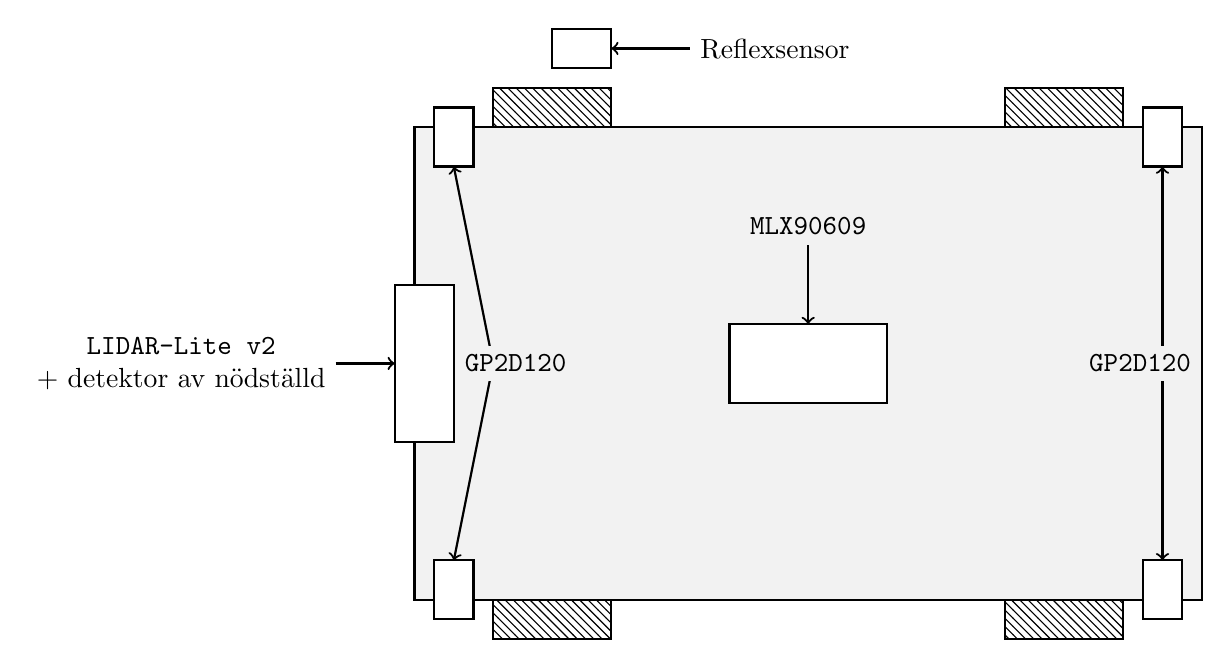
\begin{tikzpicture}[scale=1,rotate=90]
		
	%Base
	\draw[thick, draw=black, fill=gray!10] (0,0) rectangle (6,10);

	%Wheels
	\draw[thick, pattern=north west lines, pattern color=black] (-.5,1) 		rectangle (0,2.5);
	\draw[thick, pattern=north west lines, pattern color=black] (-.5,7.5) 	rectangle (0,9);
	\draw[thick, pattern=north west lines, pattern color=black] (6,1) 		rectangle (6.5,2.5);
	\draw[thick, pattern=north west lines, pattern color=black] (6,7.5) 		rectangle (6.5,9);
	
	%Sensors
	\draw[thick, draw=black, fill=white] (-.25,.25) 		rectangle (.5,.75);
	\draw[thick, draw=black, fill=white] (-.25,9.25) 	rectangle (.5,9.75);
	\draw[thick, draw=black, fill=white] (5.5,.25) 		rectangle (6.25,.75);
	\draw[thick, draw=black, fill=white] (5.5,9.25) 		rectangle (6.25,9.75);
	\draw[thick, draw=black, fill=white] (2,10.25) 		rectangle (4,9.5);
	\draw[thick, draw=black, fill=white] (2.5,4) 		rectangle (3.5,6);
	\draw[thick, draw=black, fill=white] (6.75,7.5) rectangle (7.25,8.25);

	\draw[thick, <-] (7,7.5) --++(0,-1) node[right] {Reflexsensor};
	
	%Arrows and text
	\draw[thick, ->]  (3,11) node[left, align=center] {\verb+LIDAR-Lite v2+ \\ + detektor av nödställd} -- (3,10.25);
	\draw[thick, <->] (0.5,0.5)  --  (5.5,0.5) node[left=-14pt,midway, fill=gray!10] {\verb+GP2D120+};
	\draw[thick, <->] (0.5,9.5) -- (3,9) node[right=-14pt,fill=gray!10] {\verb+GP2D120+} -- (5.5,9.5);
	\draw[thick, ->] (4.5,5) node[above] {\verb+MLX90609+} -- (3.5,5);
	\end{tikzpicture}
	
\end{document}
